%\documentclass[a4paper,12pt,final,twoside]{scrartcl}
\setcounter{secnumdepth}{3}
\setcounter{tocdepth}{5}

\usepackage[utf8]{inputenc}
\usepackage[T1]{fontenc}
\linespread{1.4}
\usepackage{dsfont}
\usepackage{amsfonts}
\usepackage{amsmath}
\usepackage{amssymb}
\usepackage{amsthm}
\usepackage{mathtools}
\usepackage{mathbbol}
\usepackage{amsmath1}
\usepackage[ngerman]{babel}
\usepackage{bibgerm}
\usepackage[pdftex]{graphicx}
%\usepackage{mathpazo}
\usepackage{floatflt}
%%\usepackage{epsfig}
\usepackage{wrapfig}
\usepackage{graphicx}
\usepackage{tabularx}
\usepackage{caption} 
\usepackage{multicol} 
\usepackage{mathrsfs}
%\usepackage{pspicture}
%\usepackage{eepic}
%\usepackage{epic}
%\usepackage{trfsigns}

%\usepackage[ansinew]{inputenc}
\usepackage{longtable,array,dcolumn}
%\usepackage{ngerman}
\usepackage{epic}
\usepackage{rotate}
\usepackage{graphpap}
\usepackage{amssymb}
\usepackage[squaren]{SIunits}
\usepackage{curves}
\usepackage{float}
\usepackage{array}
\usepackage{enumerate}
\usepackage{marvosym}
\usepackage{slashed}%für feynmanslsash
\usepackage[breaklinks,pdfborder={0 0 0}]{hyperref}
\usepackage{ulem}	%angeblich funktioniert dann
\let\underbar\uline	%underbar in math auch bei greek letters
\usepackage{multirow}
%\usepackage{multicolumn}
\usepackage{enumitem}


\setlength{\parskip}{12pt}
\setlength{\parindent}{0mm}
%\newcommand{\grad}{\ensuremath{^{\circ}}
%\renewcommand{\figurename}{Abb.}		% mit usepackage caption2
%\renewcommand{\captionfont}{\small \itshape}	% mit usepackage caption2
%\setkomafont{caption}{\small \itshape}		%sollte mit caption im userpackage funktionieren
%\setkomafont{captionlabel}{\small , \itshape}	%sollte mit caption im userpackage funktionieren
\captionsetup{font = {small, sf}} %mit it anstelle von sf gibts kusiv

\date{2009-20-10}
\newcommand{\kreis}[1]{
 \qbezier(-#1,0)(-#1,#1)(0,#1)
  \qbezier(0,#1)(#1,#1)(#1,0)
  \qbezier(#1,0)(#1,-#1)(0,-#1)
  \qbezier(0,-#1)(-#1,-#1)(-#1,0)}
\newcommand{\s}{\ \big| \ }
\newcommand{\lo}{\left <}
\newcommand{\ro}{\ri >}
\newcommand{\g}{&=&}

\newcommand{\ham}{\mathcal H}
\newcommand{\hil}{\mathscr H}
\newcommand{\fok}{\mathscr F}
\newcommand{\wh}{\widehat}
%\newcommand{\left}{\left}
\newcommand{\ri}{\right}
\newcommand{\Sp}{\text{Sp}}
\newcommand{\babsatz}{\par \begingroup \leftskip=2cm}
\newcommand{\eabsatz}{\par\endgroup}

\newcommand{\D}{\text{\itshape D}}
\newcommand{\Lr}{\mathcal L }%\textit{L}}
\newcommand{\rot}{\text{rot}}
\newcommand{\divergenz}{\text{div}}
\newcommand{\grad}{\text{grad}}
\newcommand{\grat}{${}^{\circ}$}
%\newcommand{\tanh}{\text{tanh}} already defined

\newcommand{\RM}[1]{\text{\MakeUppercase{\romannumeral #1}}}
\newcommand{\dell}{\partial}
\renewcommand{\div}{\operatorname{div}}
\newcommand{\I}{\dot{\text{\i\!\i}}}
\newcommand{\e}{\mathrm{e}}
\newcommand{\ket}[1]{\mid\!\!\!\,\,{#1}\rangle}
\newcommand{\bra}[1]{\langle{#1}\!\!\!\,\,\mid}
\newcommand{\braket}[2]{\langle{#1}\!\!\!\,\,\mid\!\!\!\,\,{#2}\rangle}
\newcommand{\bracket}[3]{\langle{#1}\!\!\!\,\,\mid\!\!\!\,\,{#2}\!\!\!\,\,\mid\!\!\!\,\,{#3}\rangle}
\newcommand{\1}{\mathds{1}}
\newcommand{\EW}[1]{\langle\!\!\,\,#1\!\!\,\,\rangle}
\newcommand{\arrowbox}[1]{-\!\!\!\!\:\text{(#1)}\!\!\!\;\;\!\!\!\rightarrow}

\newcommand{\ketI}[1]{\ket{#1}_{\!\!\;\text{I}}}
\newcommand{\ketII}[1]{\ket{#1}_{\!\!\;\text{II}}}
\newcommand{\ketIII}[1]{\ket{#1}_{\!\!\;\text{III}}}
\newcommand{\braI}[1]{\,\!_{\text{I}\!\!\;}\bra{#1}}
\newcommand{\braII}[1]{\,\!_{\text{II}\!\!\;}\bra{#1}}
\newcommand{\braketI}[2]{\,_{\text{I}\!\!\;}\braket{#1}{#2}_{\!\!\;\text{I}}\,}
\newcommand{\braketII}[2]{\,_{\text{II}\!\!\;}\braket{#1}{#2}_{\!\!\;\text{II}}\,}
\newcommand{\braketIII}[2]{\,_{\text{III}\!\!\;}\braket{#1}{#2}_{\!\!\;\text{III}}\,}
\newcommand{\bracketI}[3]{\,_{\text{I}\!\!\;}\bracket{#1}{#2}{#3}_{\!\!\;\text{I}}\,}
\newcommand{\bracketII}[3]{\,_{\text{II}\!\!\;}\bracket{#1}{#2}{#3}_{\!\!\;\text{II}}\,}


\newcommand{\up}{\ket{\uparrow}}
\newcommand{\updg}{\bra{\uparrow}}
\newcommand{\down}{\ket{\downarrow}}
\newcommand{\downdg}{\bra{\downarrow}}
\newcommand{\upup}{\ket{\uparrow\uparrow}}
\newcommand{\updown}{\ket{\uparrow\downarrow}}
\newcommand{\downup}{\ket{\downarrow\uparrow}}
\newcommand{\downdown}{\ket{\downarrow\downarrow}}

\newenvironment{itemize1}{\begin{itemize}[leftmargin=5mm,itemsep=-1ex,topsep=-1ex]}{\end{itemize}}

%\usepackage[left=2cm,right=2cm,top=1cm,bottom=1cm,includeheadfoot]{geometry}

\usepackage{fancyhdr}
\pagestyle{fancy}{\fancyhf{}
\fancyhead[LO,RE]{\footnotesize \rightmark}
\fancyfoot[C]{\footnotesize -$\,$\thepage$\;$-}
\renewcommand{\headrulewidth}{0.4pt}
\renewcommand{\footrulewidth}{0pt}}

\fancypagestyle{plain}{\fancyhf{}
\renewcommand{\headrulewidth}{0.4pt}
\fancyfoot[C]{\footnotesize -$\,$\thepage$\,$-}}

\usepackage{titlesec}
\titleformat{\section}[display]{\sffamily\bfseries\Huge\center}{Kapitel \thetitle:}{1ex}{}{}
\newcommand{\kapitel}[2]{$\;$\vspace{-1.5cm} \section[#1]{#2} \rule{17cm}{0.4pt}\vspace{3cm}}
\titleformat{\paragraph}[hang]{\sffamily\bfseries}{\thetitle:}{0ex}{\vspace{-0.15cm}}{\vspace{0.5cm}}

\title{ \vspace{1.5cm}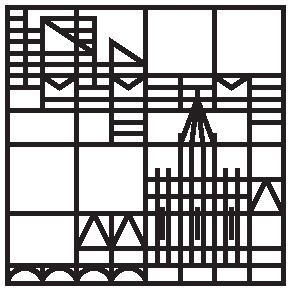
\includegraphics[width=5cm]{logo}
\\ \Large Universität Konstanz  \\ \vspace{4ex} \huge 
Skript zur Vorlesung\\ Höhere Quantentheorie und Elektrodynamik
\\ \vspace{4ex} \Large Prof. Dr. Wolfgang Belzig 
\\ Version vom 30. Juli 2012 \\ \vspace{4.5cm}
\normalsize Ursprünglichen Mitschrift von Birte Heinze im WS 09/10 \\ Ausführliche Überarbeitung von Tobias Lohse im WS 11/12 \vspace{-10cm}}
\author{}
\date{}
%\begin{document}

\subsection*{Einleitung} \vspace{-.5cm}\addcontentsline{toc}{subsection}{\qquad\,\! Einleitung}\markboth{Einleitung}{Einleitung}
Die moderne Quantentheorie stellt heutzutage einen der wichtigsten und umfänglichsten Bereiche der Physik dar, welcher in verschiedensten Bereichen der aktuellen Forschung von Bedeutung ist. In der Tat gibt es nur wenige Bereiche der modernen Physik, in denen Quantenmechanische Effekte keinerlei Rolle spielen. Ein gutes Verständnis der Systematik, mathematischen Formulierung und Anwendung der Quantentheorie ist daher eine absolut notwendige Vorraussetzung für ein Verständnis von moderner Physik. 

Dieses Skript und die Vorlesung auf der es beruht sollen einen Einblick in die Vielfalt der verschiedensten Bereiche der Quantentheorie bieten und eine Grundlage für das Verständnis der Systematik dieser verschiedenen Teilbereiche bieten, auf deren Basis eine Einordnung und ein grundlegendes Verständnis der Teilbereiche moderner Quantenphysik möglich sind. Es werden grundlegende Kenntnisse der klassischen Mechanik, Elektrodynamik und Speziellen Relativitätstheorie sowie der einfachen Quantenmechanik und deren mathematischen Formalismen vorausgesetzt. Der Inhalt ist in Vier Kapitel gegliedert:

\begin{itemize1}
	\item Im ersten Kapitel sollen zunächst die Grundlagen der einfachen Quantenmechanik wiederholt werden, danach soll die Addition von Drehimpulsoperatoren, die zeitabhängige Störungstheorie und die quantenmechanische Streutheorie näher erläutert werden, die in diesen Abschnitten erläuterten Theorien sind insbesondere für das Verständnis der Grundlagen der Festkörperphysik wichtig, spielen aber auch in vielen anderen Anwendungen der Quantenphysik eine wichtige Rolle. Im nächsten Abschnitt soll ein Einblick in die Formulierung und Herleitung der Quantendynamik nach Feynman mittels Propagatoren gegeben werden, welche eine wichtige Grundlage für die Formulierung der Quantenfeldtheorie darstellt. Abschließend soll in diesem ersten Kapitel dann noch kurz auf den Messprozess und die Wahrscheinlichkeitsinterpretation der Quantenmechanik eingegangen werden, welche für das Verständnis von Quantenstatistik und Quanteninformationstheorie eine wichtige Rolle spielen. 
	\item Im zweiten Kapitel soll auf die relativistische Formulierung der Elektrodynamik eingegangen werden. Dazu werden wir zunächst die Grundlagen der Speziellen Relativitätstheorie (SRT) und deren Formalismus wiederholen und danach die Elektrodynamik in diesem Formalismus formulieren. Außerdem soll auf den Lagrangeformalismus der SRT eingegangen werden, welcher die Grundlage für die Formulierung relativistischer Quantenfeldtheorien darstellt. 
	\item Es soll nun im dritten Kapitel auf die Relativistische Quantenmechanik eingegangen werden. Insbesondere sollen die Klein-Gordon-Gleichung und die Dirac-Gleichung Motiviert und Erläutert werden und der Formalismus für die Relativistische Quantenmechanik formuliert werden. Die relativistische Quantenmechanik spielt insbesondere eine bedeutende Rolle, insofern sie den Spin einführt und damit im nichtrelativistischen Grenzfall in die Pauli-Gleichung übergeht. Außerdem stellt sie die Grundalge für jegliche Elementarteilchentheorien dar und motiviert die Notwendigkeit einer Quantenfeldtheorie. 
	\item Im letzten Kapitel soll schlussendlich eine Einführung in die Quantefeldtheorie gegeben werden. Dabei wird zunächst der Formalismus der Quantenfeldtheorie und die Darstellung von Operatoren in zweiter Quantisierung eingeführt. Abschließend soll auf die Feldquantisierung der Diractheorie und des Strahlungsfeldes eingegangen werden. Mit der Quantenfeldheorie ist die Grundlage für die Quantenelektrodynamik und Quantenstatistik und damit  der modernen theoretischen Festkörperphysik gelegt außerdem stellt sie die Grundlage für die Formulierung der Quantenchromodynamik und der gesamten modernen theoretischen Elementarteilchentheorie dar. 
\end{itemize1}

Das folgende Diagramm soll die Zusammenhänge der verschiedenen quantenmechanischen Theorien und die Einordnung in Teilbereiche der Physik verdeutlichen: 

\begin{figure}[b!]\center
\includegraphics[width=.95\linewidth]{Figs/overview.pdf}
\end{figure}

%\end{document}